\documentclass[12pt]{article}
\usepackage[utf8]{inputenc}
\usepackage{multicol}
\usepackage{fancyhdr}
\usepackage{gensymb}
\usepackage{graphicx}
\usepackage{listings}
\usepackage{color}
\usepackage[margin=1in]{geometry}


\lstset{frame=tb,
  language=Matlab,
  aboveskip=3mm,
  belowskip=3mm,
  showstringspaces=false,
  columns=flexible,
  basicstyle={\small\ttfamily},
  numbers=none,
  numberstyle=\tiny\color{gray},
  keywordstyle=\color{blue},
  commentstyle=\color{dkgreen},
  stringstyle=\color{mauve},
  breaklines=true,
  breakatwhitespace=true,
  tabsize=3
}
\definecolor{dkgreen}{rgb}{0,0.6,0}
\definecolor{gray}{rgb}{0.5,0.5,0.5}
\definecolor{mauve}{rgb}{0.58,0,0.82}

\begin{document}

\begin{titlepage}
    \begin{center}
        \vspace*{1cm}
            
        \LARGE
        \textbf{Determination of the Aerodynamic Performance of a Low‐Speed
Airfoil based on Pressure Distribution Measurements}
            
        \vspace{0.5cm}
        \Large
        Aerodynamics and Propulsion
Laboratory 
            
        \vspace{1.5cm}
        \large
        \textbf{Section 2}\\
        \normalsize\vspace{15 pt}
        Tyler Cascalho Cox\\
            
        \vfill
            
            
        \vspace{0.8cm}
            
            
        \Large
        Iowa State University\\
        Undergraduate Aerospace Engineering
        
            
    \end{center}
\end{titlepage}


\pagestyle{fancy}
\fancyhead[LE,RO]{\normalsize Section 2}
\fancyhead[RE,LO]{\normalsize Aerodynamic Performance of a Low-Speed Airfoil }
\fancyfoot[CE,CO]{\leftmark}
\fancyfoot[LE,RO]{\thepage}


\section*{Abstract}
In this report the aerodynamic performance of a GA(W)-1 airfoil is analysed at various angles of attack. Pressure taps around the airfoil are used to find the pressure distribution. Which is used to find the lift, drag and moment coefficients at each of the angles of attack. This is then used to determine the movement of the stagnation point as angle of attack is varied and the angle of attack at which flow separation and stall start at.


\newline
\section*{Variables and Symbols}
\(P\) - Pressure (Pa) \newline\newline
\(C_p\) - Pressure Coefficient \newline\newline
\(P_A\) - Contraction Section Pressure (Pa) \newline\newline
\(P_E\) - Inlet Pressure (Pa) \newline\newline
\(\rho\) - Density of Air \(\left(\frac{\mbox{kg}}{{\mbox{m}}^3}\right)\) \newline\newline
\(\alpha\) - Angle of Attack (Degrees) \newline\newline
\(C_D\) - Drag Coefficient\newline\newline
\(C_L\) - Lift Coefficient\newline\newline
\(C_M\) - Moment Coefficient\newline\newline
\(D\) - Drag Force (N)\newline\newline
\(L\) - Lift Force (N)\newline\newline
\(M_{LE}\) - Leading Edge Moment (Nm)\newline\newline
\(K\) - Calibration Constant \newline\newline

\newline
\newpage
\tableofcontents
\label{sec:Abstract}
\addcontentsline{toc}{section}{\nameref{\hspace{10 pt} Abstract}}
\newpage
 

\section{Introduction}
For this experiment a GA(W)-1 airfoil has been outfitted with 43 pressure taps and tested at nine different angles of attack with the wind tunnel velocity held constant. Three pressure transducers were attached to pressure taps around the airfoil to collect the raw data. The data was time-averaged and then  used to obtain plots of the lift, drag, moment, and pressure coefficients vs. angle of attack.
\newpage
\section{Theory}
\subsection{The Closed Loop Wind Tunnel}
The closed loop wind tunnel is comprised of seven main sections/components. These are the Test Section, Contraction Section, Diffuser Section, Settling Chamber, Screens/Flow management, Cooling System, and a Motor/Fan. These are depicted below (Figure 1). 

    \begin{figure}[h]
        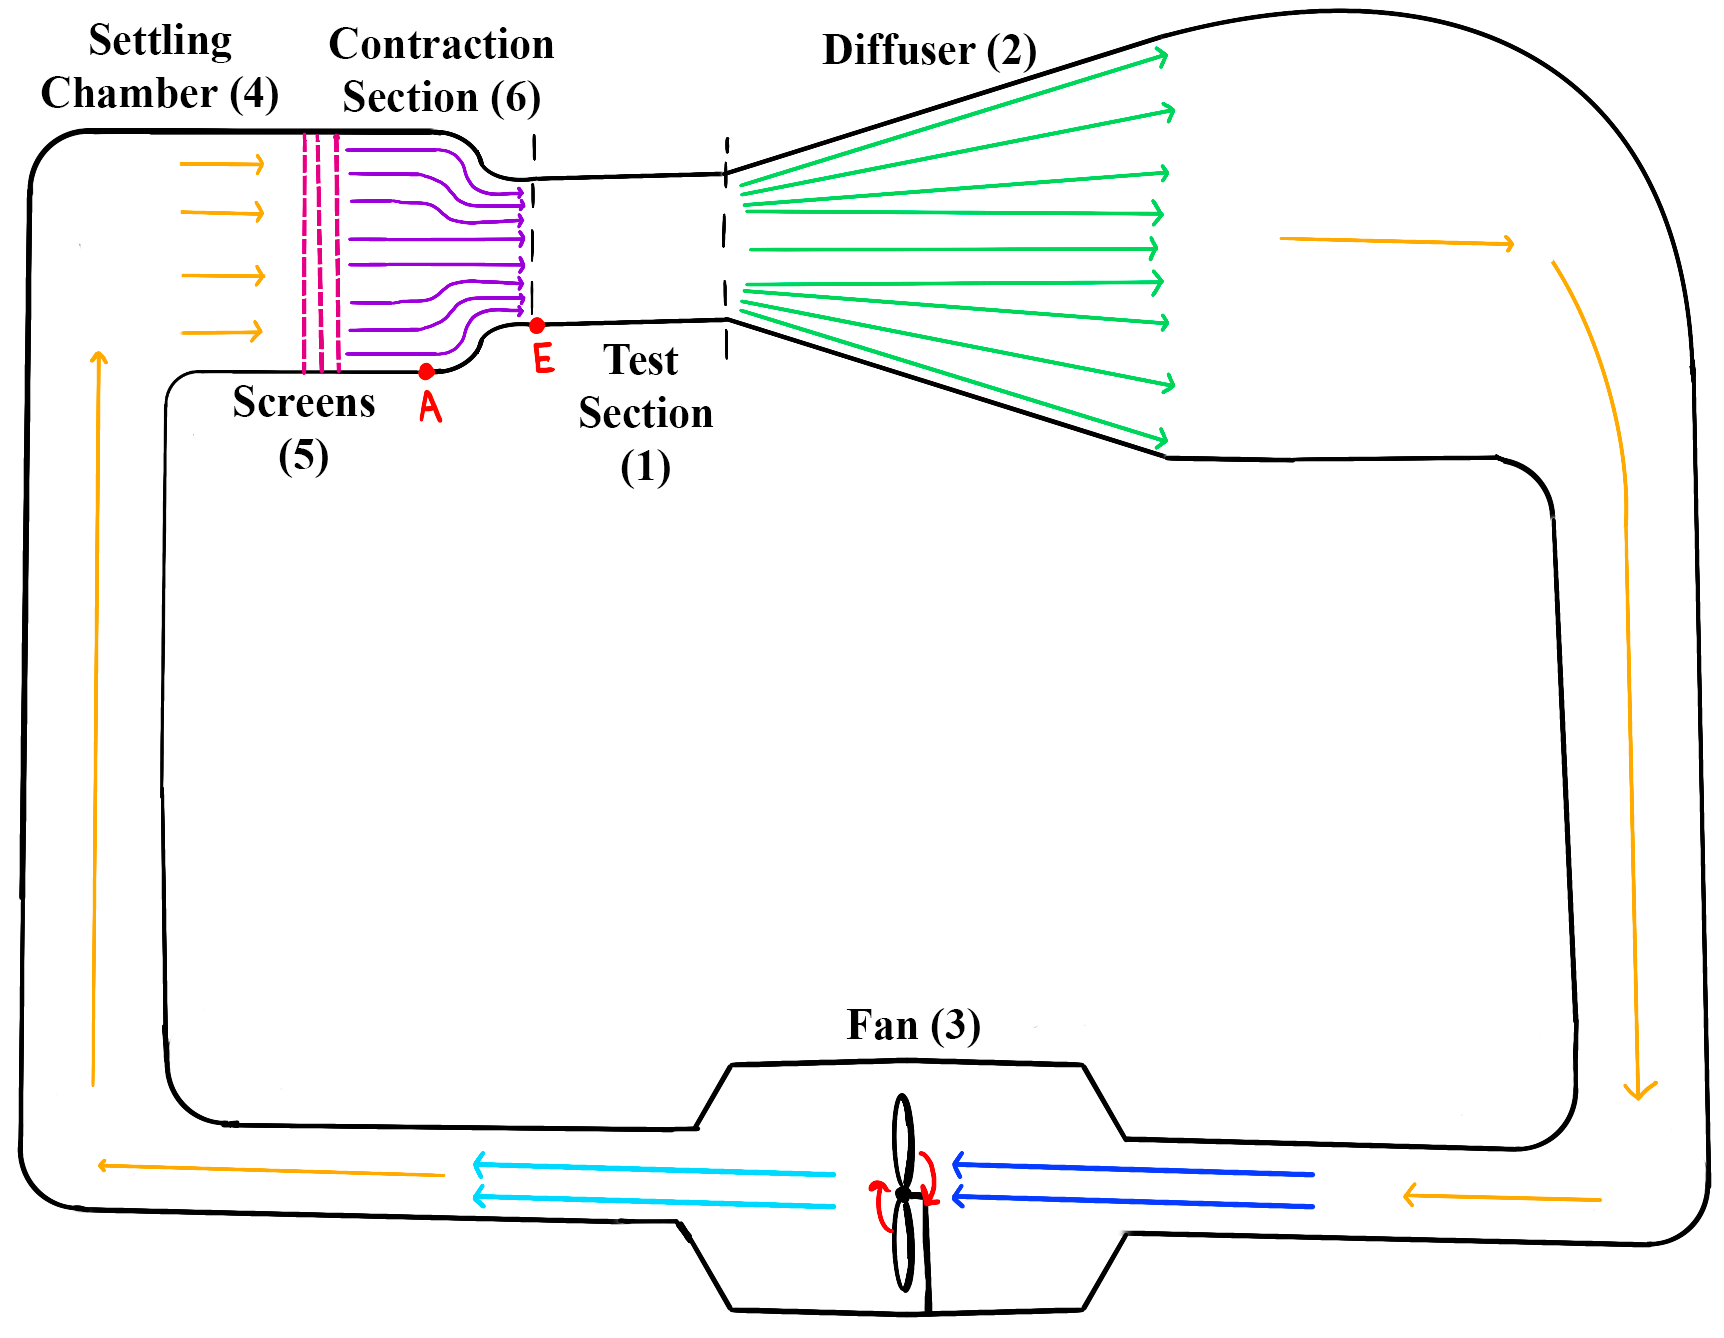
\includegraphics[width=16 cm]{Figure1.png}
        \centering
        \label{Figure 1}
        \caption{Closed Loop Wind Tunnel}
    \end{figure}
A closed loop wind tunnel is a tool often used in field of Aerospace to determine the flow field around objects of interest (i.e. things like cars, airfoils, ect). In a low speed wind tunnel things are particularly nice since it satisfies the criteria required for Bernoulli's equation to be applicable. This allows for easier measurement of the flow velocity within the wind tunnel and also results in simpler flow fields in general.

\subsection{Bernoulli's equation and The Pitot-Static Probe}
There are three criteria that must be satisfied for Bernoulli’s equation to be valid. These criteria are as follows, a given flow must be steady (velocity at a point cannot change with time), it must be incompressible (density along a steamline must remain constant), and friction due to viscous forces must be negligible. In a low speed wind tunnel these criteria are satisfied. Now, Bernoulli's equation is as follows:
\begin{equation}
    p+\frac{1}{2}\rho v^2+\rho g h = \mbox{constant}
\end{equation}
For our purposes we can ignore the \(\rho g h\) term since we are taking our flow inside the area of interest to be horizontal. This gives us the following:
\begin{equation}
    P_T = p+\frac{1}{2}\rho v^2 
\end{equation}
Where \(P_T\) represents total pressure, which is constant. We can then solve this equation for the velocity of the flow.
\begin{equation}
    v = \sqrt{\frac{2\left(P_T - p\right)}{\rho}}
\end{equation}
This means that if we have the total pressure \(P_T\) (a.k.a stagnation pressure) and the static pressure \(p\) then we can find the velocity of the flow. Fortunately, we have measurement tool that does just that and it's called a pitot-static probe (Figure 2).
    \begin{figure}[h]
        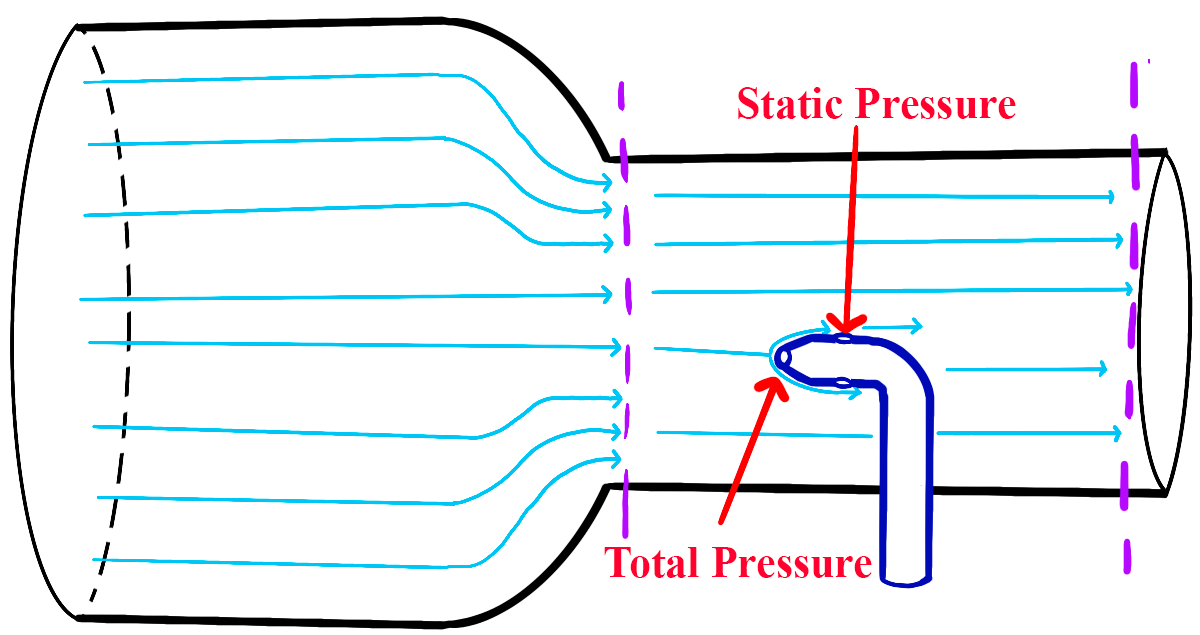
\includegraphics[width=14cm]{Figure2.png}
        \centering
        \label{Figure 2}
        \caption{Pitot-Static Probe}
    \end{figure}

Unfortunately, the pitot-static probe is quite intrusive and disrupts the flow quite a bit and thus cannot be used to determine flow velocity while trying to find the flow profile of another object. Now, the alternate method to this is to take static pressure measurements at points A and E as shown in Figure 1. In theory the pressure difference between A and E should be linearly related to dynamic pressure in the test section. Which means we can find a calibration constant relating the dynamic pressure to the pressure difference between points A and E.

\subsection{The Calibration Constant}
As discussed above there should exist a calibration constant that when multiplied by the pressure difference between points A and E (Figure 1) you get dynamic pressure inside the test section. To find this constant we need to start with Bernoulli's equation. 
\[P_i = p_i+q_i\]
Applying this to our points A and E
\[P = p_A+q_A = p_E + q_E\]
Now we need to account for the pressure loss due to the boundary layer effect at A and E
\[P_A = p_A + q_A = p_E+q_E+(P_A -P_E )\]
Now we define a pressure loss coefficient
\[C_1 = \frac{P_A -P_E }{q_E}\]
Substituting this into the equation above:
\begin{equation}
    p_A-p_E=q_E+q_EC_1-q_A
\end{equation}

Lets let \(A_A, A_E, \mbox{ and }A_T\) denote the cross sectional area at points A, E, and the test section respectively. We then equate the mass flow rate equations using the conservation of mass.
\[\rho_A v_A A_A = \rho_E v_E A_E = \rho_T v_T A_T\]
Since this is a low-speed flow, we can assume that it is inviscid. Which means that \( \rho_A =\rho_E=\rho_T \) and therefore get the following equation:
\[\ v_A A_A =  v_E A_E = v_T A_T\]
After squaring and multiplying by \(\frac{\rho}{2}\) we get the following equation:
\[\frac{1}{2}\rho_A {v_A}^2 {A_A}^2 = \frac{1}{2}\rho_E {v_E}^2 {A_E}^2=\frac{1}{2}\rho_T {v_T}^2 {A_T}^2\]
Simplifying:
\[q_A {A_A}^2 = q_E {A_E}^2 = q_T {A_T}^2\]
Defining more coefficients:
\[C_2 = \frac{{A_E}^2}{{A_A}^2} \mbox{ and } C_3 = \frac{{A_T}^2}{{A_E}^2}\]
\[\rightarrow  q_A = C_3 q_E \mbox{ and } q_E = C_3 q_T\]
Now plugging this into (4) gives:
\[p_A-p_E = C_3 q_T +C_1 C_3 q_T - C_2 C_3 q_T = (1+C_1-C_2)C_3 q_T=C q_T\]\
\begin{equation}
    \rightarrow K=\frac{1}{C} = \frac{q_T}{p_A-p_E} =\frac{q_T}{\Delta p}
\end{equation}
Where K is the calibration constant.
\subsection{Estimating the Pressure Integral}
The lift, drag, and moment coefficients can be calculated by integrating the distribution of surface pressure around the airfoil. If we define the i-th panel as bounded by the i-th and i+1-th taps, then the pressure \(p_{i+1/2}\) (acting on the i-th panel) can be calculated using
\[p_{i+1/2}=\frac{1}{2}\left( p_{i} + p_{i+1}\right)\]
Then we assume the pressure variation is constant and define
\[\Delta x_i = x_{i+1} - x_i\]
\[\Delta y_i = y_{i+1} - y_i\]
From equations 1 and 2 we can define the normal and axial components acting on the i-th panel (with the prime indicating force per unit span):
\[\delta {N_i}^{'}=p_{i+1/2}\Delta x_i\]
\[\delta {A_i}^{'}=p_{i+1/2}\Delta y_i\]
These values are visualized on the airfoil surface in the following figure:
    \begin{figure}[h]
        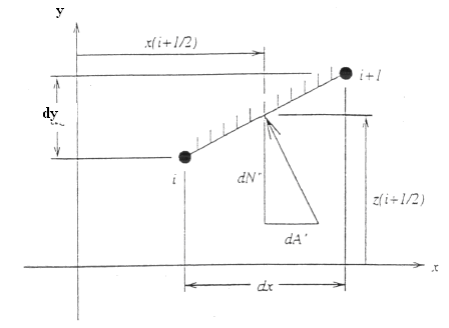
\includegraphics[width=12 cm]{pic3.PNG}
        \centering
        \caption{Discrete representation of the airfoil surface element}
    \end{figure}
    The moment contribution from the i-th panel to the total leading edge moment can be determined using a similar method (positive in the pitch-up direction):

\[\delta {M^'}_{LE,i} = r \times \delta F_i = \left( x_{i+1/2}i+y_{i+1/2}k \right) \times  \left( \delta {{A_{i}}^'} i +\delta {{N_{i}}^'} k \right)\]

Which can be simplified to
\[\delta {M^'}_{LE,i} = -\left( p_{i+1/2}\Delta x_i \right)x_{i+1/2}-\left( p_{i+1/2} \Delta y_i \right) y_{i+1/2}\]

With
\[x_{i+1/2} = \frac{1}{2} \left( x_i +x_{i+1} \right)\]
\[y_{i+1/2} = \frac{1}{2} \left( y_i +y_{i+1} \right)\]

The expressions for the differential force and moment on each panel can now be integrated over the airfoil surface by using the total sums:

\[{N^'}=\sum^N_{i=1} \delta {N^'}_i = \sum^N_{i=1} p_{i+1/2} \Delta x_i\]

\[{A^'}=\sum^N_{i=1} \delta {A^'}_i = -\sum^N_{i=1} p_{i+1/2} \Delta y_i\]

\[{M^'}_{LE} = \sum^N_{i=1} \delta {M^'}_{LE} = -\sum^N_{i=1}\left( p_{i+1/2} \Delta x_i \right)x_{i+1/2} - \sum^N_{i=1} \left( p_{i+1/2} \Delta y_i \right) y_{i+1/2}\]

Using these values we can determine the lift and drag per unit span:
\[{L^'} = {N^'} \cos (\alpha) - {A^'} \sin (\alpha) \]

\[{D^'} = {N^'} \sin (\alpha) + {A^'} \cos (\alpha) \]

\[C_L = \frac{{L^'}}{K(P_A-P_E)}\]

\[C_D = \frac{{D^'}}{K(P_A-P_E)}\]

\[C_M = \frac{{M^'}_{LE}}{K(P_A-P_E)}\]

\newpage
\section{Experimental Setup}
\subsection{General Description}
The low speed wind tunnel and a GA(W)-1 airfoil with 43 pressure taps in it were used to find the pressure distribution at the following angles of attack: \([ -4\degree, 0\degree, 4\degree, 6\degree, 8\degree, 10\degree, 12\degree, 14\degree, 16\degree]\). A wind tunnel motor frequency of 15 Hz was used, which produces a test section flow velocity of about \(22 \hspace{2 pt}\frac{\mbox{m}}{\mbox{s}}\)(Figure 17). The pressure taps were hooked up to 3 pressure transducers which were then hooked up to the computer to record the results. At each angle of attack 1000 pressure measurements for each pressure tap was made. During the analysis these were then averaged for each angle of attack. The values of \(P_A\) and \(P_E\) were used to calculate the dynamic pressure of the system using Bernoulli’s equation (Section 2.3). Then the method described in Section 2.4 was used to determine the lift, drag, and moment coefficients.
    \begin{figure}[h]
        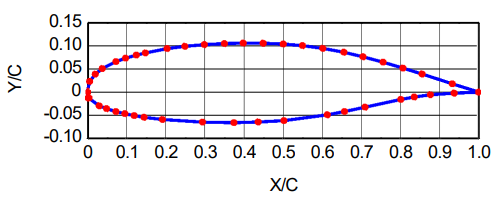
\includegraphics[width=16 cm]{air.PNG}
        \centering
        \caption{GA(W)-1 Airfoil with Pressure Taps (Red)}
    \end{figure}



\subsection{Case Study}
The lab was at NTP during the experiment
\begin{itemize}
    \item \(P_{ntp} = 1 \hspace{3 pt}\mbox{atm}\)
    \item  \(\rho_{ntp} = 1.204  \hspace{3 pt}\frac{\mbox{kg}}{{\mbox{m}}^3}\)
    \item \(T_{ntp} = 20 \hspace{3 pt}\degree\mbox{C}\)
\end{itemize}

\newpage
\section{Results}
\subsection{\(C_P\) distribution for \(\alpha = -4\degree\)}
    \begin{figure}[h]
        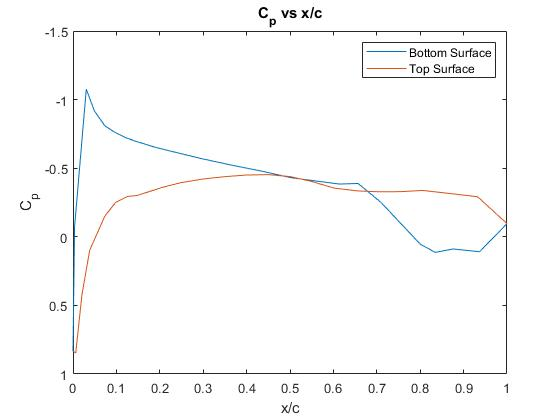
\includegraphics[width=16 cm]{-4.jpg}
        \centering
        \caption{\(C_P\) distribution for \(\alpha = -4\degree\)}
    \end{figure}
    
    \newpage
    \subsection{\(C_P\) distribution for \(\alpha = 0\degree\)}
    \begin{figure}[h]
        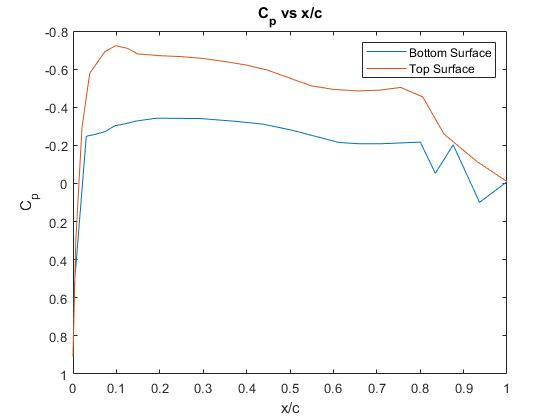
\includegraphics[width=16 cm]{0.jpg}
        \centering
        \caption{\(C_P\) distribution for \(\alpha = 0\degree\)}
    \end{figure}
    
    \newpage
    \subsection{\(C_P\) distribution for \(\alpha = 4\degree\)}
    \begin{figure}[h]
        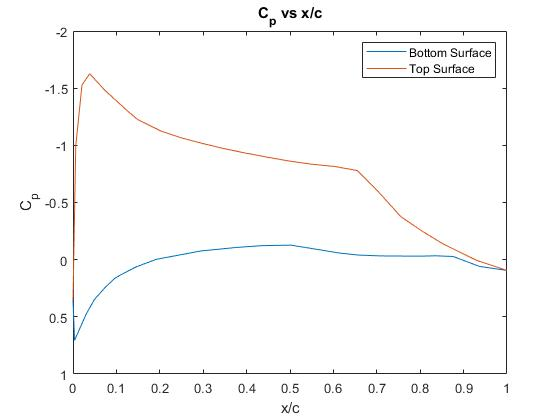
\includegraphics[width=16 cm]{4.jpg}
        \centering
        \caption{\(C_P\) distribution for \(\alpha = 4\degree\)}
    \end{figure}
    
        \newpage
    \subsection{\(C_P\) distribution for \(\alpha = 6\degree\)}
    \begin{figure}[h]
        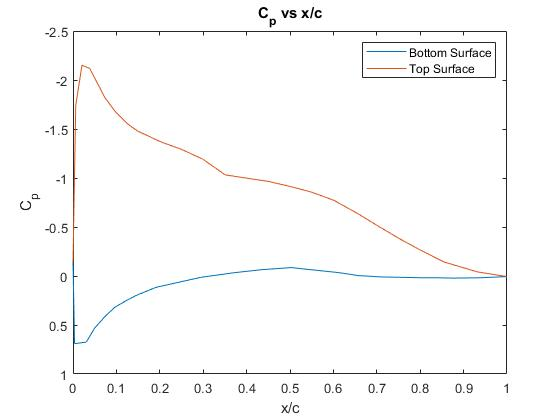
\includegraphics[width=16 cm]{6.jpg}
        \centering
        \caption{\(C_P\) distribution for \(\alpha = 6\degree\)}
    \end{figure}
    
        \newpage
    \subsection{\(C_P\) distribution for \(\alpha = 8\degree\)}
    \begin{figure}[h]
        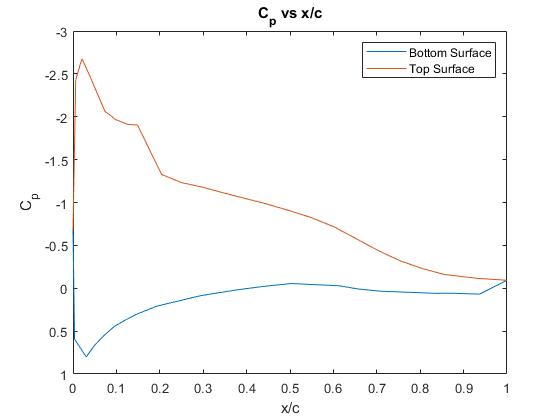
\includegraphics[width=16 cm]{8.jpg}
        \centering
        \caption{\(C_P\) distribution for \(\alpha = 8\degree\)}
    \end{figure}

    \newpage
    \subsection{\(C_P\) distribution for \(\alpha = 10\degree\)}
    \begin{figure}[h]
        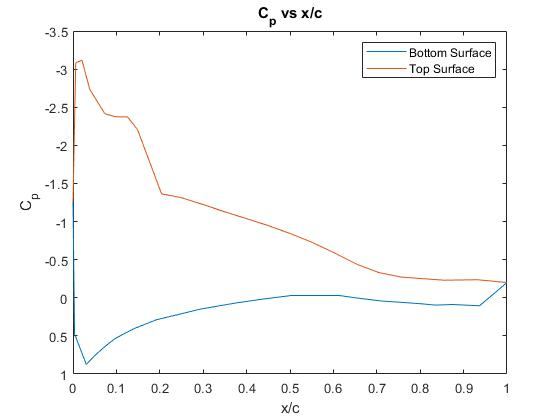
\includegraphics[width=16 cm]{10.jpg}
        \centering
        \caption{\(C_P\) distribution for \(\alpha = 10\degree\)}
    \end{figure}
    
        \newpage
    \subsection{\(C_P\) distribution for \(\alpha = 12\degree\)}
    \begin{figure}[h]
        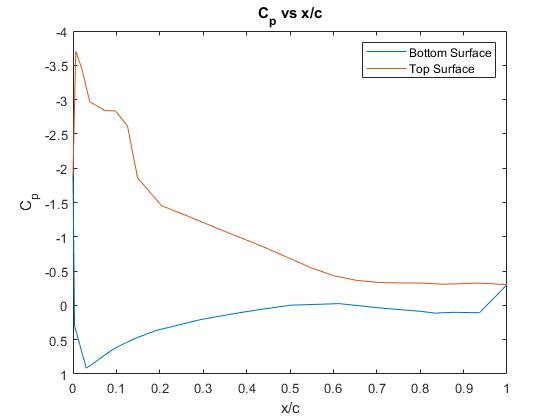
\includegraphics[width=16 cm]{12.jpg}
        \centering
        \caption{\(C_P\) distribution for \(\alpha = 12\degree\)}
    \end{figure}
    
        \newpage
    \subsection{\(C_P\) distribution for \(\alpha = 14\degree\)}
    \begin{figure}[h]
        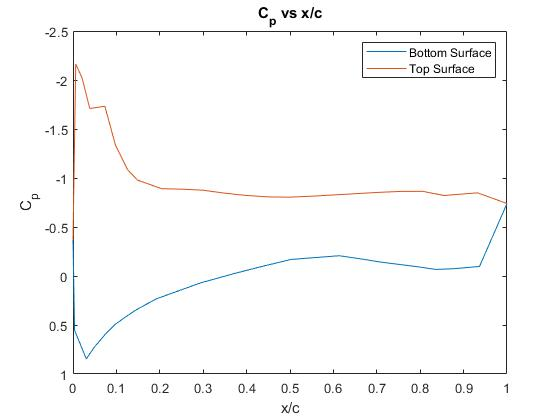
\includegraphics[width=16 cm]{14.jpg}
        \centering
        \caption{\(C_P\) distribution for \(\alpha = 14\degree\)}
    \end{figure}
    
        \newpage
    \subsection{\(C_P\) distribution for \(\alpha = 16\degree\)}
    \begin{figure}[h]
        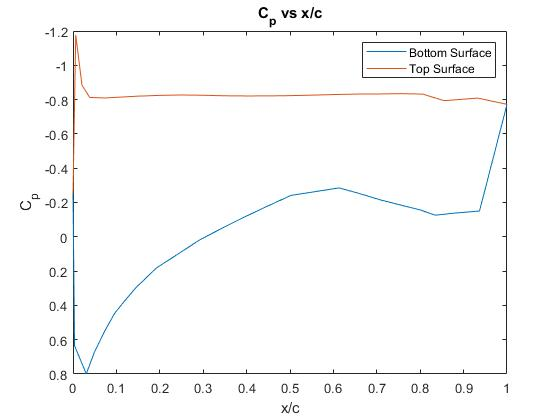
\includegraphics[width=16 cm]{16.jpg}
        \centering
        \caption{\(C_P\) distribution for \(\alpha = 16\degree\)}
    \end{figure}
    
        \newpage
    \subsection{\(C_L\) variation with changes to \(\alpha\)}
    \begin{figure}[h]
        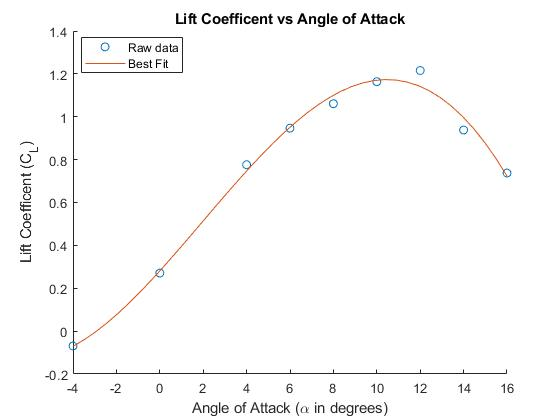
\includegraphics[width=16 cm]{CL.jpg}
        \centering
        \caption{\(C_L\) variation with changes to \(\alpha\)}
    \end{figure}

            \newpage
    \subsection{\(C_D\) variation with changes to \(\alpha\)}
    \begin{figure}[h]
        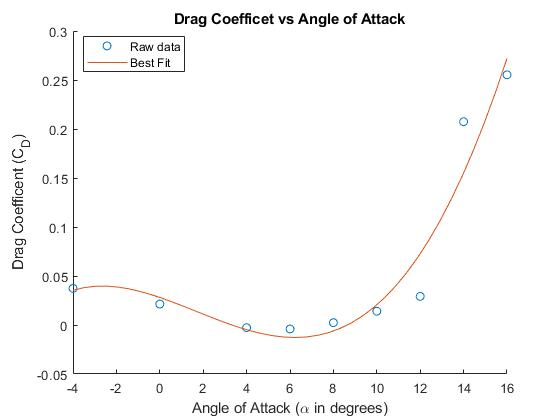
\includegraphics[width=16 cm]{Cd.jpg}
        \centering
        \caption{\(C_D\) variation with changes to \(\alpha\)}
    \end{figure}

            \newpage
    \subsection{\(C_M\) variation with changes to \(\alpha\)}
    \begin{figure}[h]
        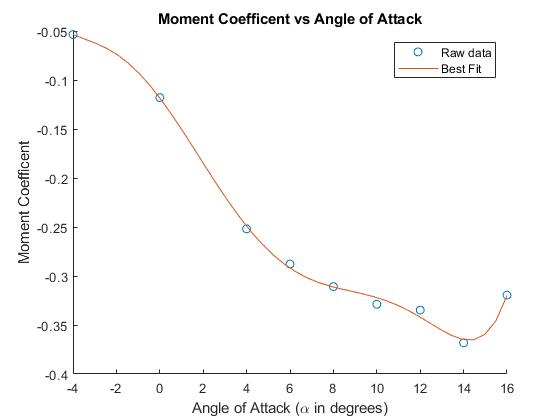
\includegraphics[width=16 cm]{Cm.jpg}
        \centering
        \caption{\(C_M\) variation with changes to \(\alpha\)}
    \end{figure}
    \newpage
\subsection{The Calibration Constant and Plot between \(q_T\) and \(\Delta p\)}
    \begin{figure}[h]
        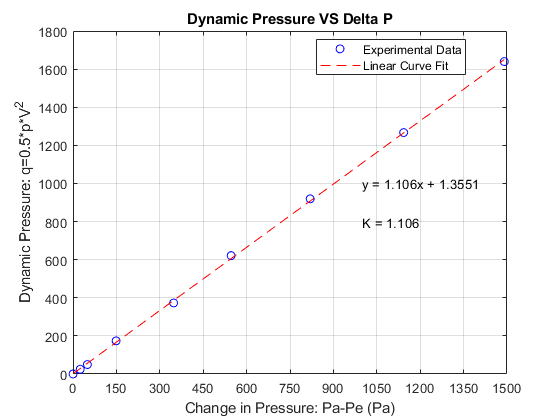
\includegraphics[width=15 cm]{Figure4.png}
        \centering
        \caption{\(q_T\) vs. \(\Delta p\)}
    \end{figure}
\newpage
\subsection{Flow Velocity vs. Motor Speed}
    \begin{figure}[h]
        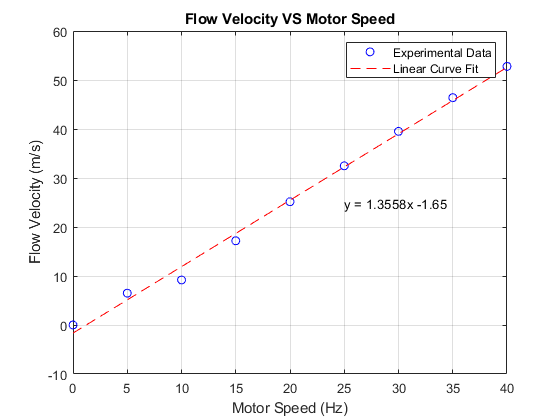
\includegraphics[width=15 cm]{Figure5.png}
        \centering
        \caption{Flow Velocity vs. Motor Speed}
    \end{figure}

\subsection{Reynolds Number}
The Re value for this experiment is as follows:
\[\mbox{Re} = \frac{\rho V c}{\mu} =  \frac{\left(1.2040 \hspace{2 pt} \frac{\mbox{kg}}{\mbox{m}^3}\right) \left(22 \hspace{3 pt}\frac{\mbox{m}}{\mbox{s}}\right) \left(0.101 \mbox{ m}\right)}{(1.81*10^{-5} \mbox{ Pa s})} = 147805.97\]

\newpage
\subsection{General Discussion of Results and of Error}
The pressure distributions obtained seem realistic and reasonable. Now, there are a few graphs that are particularly interesting. In Figure 2 the pressure on the bottom surface sharply decreases overtaking the pressure on the top surface. This is the only graph in which this happens and it is because the airfoil was at a negative angle of attack thus causing a pressure increase on the top of the airfoil and a decrease in pressure on the bottom surface of the airfoil. Another interesting graph is Figure 9 where there is a large zone on the top surface of the airfoil with constant pressure. The cause of this apparent constant pressure is the flow separating from the airfoil. This separation appears to start at \(\alpha = 10\degree\) (Figure 7) and is exacerbated at \(\alpha = 16 \degree\) (Figure 10). 
\newline
\newline
Another interesting result, attained from the pressure distribution graphs, is the movement of the stagnation point on the airfoil as the angle of attack is varied. These estimations can be found under A.4 Figure 17. There it is shown that the stagnation point moves back along the bottom surface of the airfoil as the angle of attack is increased, which makes sense.
\newline
\newline
As for the graphs for the Lift, Drag, and Moment coefficient, they all seem reasonable and there are no apparent warning signs that indicate there was an error in their calculation. We can also estimate the angle of attack at which stall occurs from our \(C_L\) vs \(\alpha\) graph (Figure 11). From this graph the angle of attack at which stall occurs at is approximately \(12 \degree\). 
\newpage
\section{Conclusion}
Pressure distribution over an airfoil is a function of the angle of attack of that airfoil. However, when flow separation occurs the pressure distribution with flatten out on a constant value. The Lift, Drag, and Moment coefficients are also functions of the angle of attack and the Lift coefficient has an angle off attack at which it drastically drops known as the stall angle. For the GA(W)-1 airfoil this occurs at approximately \(\alpha = 12 \degree\). Similarly, flow separation for the GA(W)-1 airfoil begins at \(\alpha = 10\degree\). 

\newpage
\section{Work Cited}
Department of Aerospace Engineering. "Lab 5 Instructions". Lab handbook. Iowa State University. Ames, Iowa. 2020. Print.
\newline

\newpage
\setcounter{section}{0}
\def\thesection{\Alph{section}}
\section{Appendix of Data Tables}
\subsection{Average Pressure Measurements}
    \begin{figure}[h]
        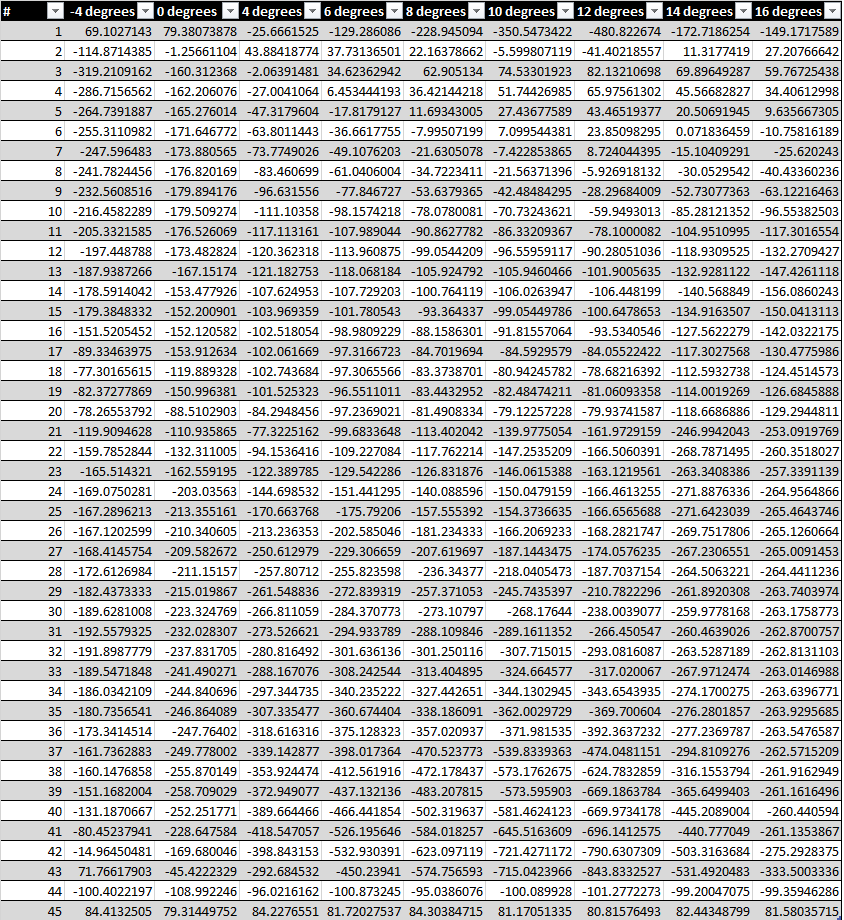
\includegraphics[width=15.4 cm]{png.png}
        \centering
        \caption{Pressure Tap Averages in (Pa)}
    \end{figure}
\newpage
\subsection{Values for \(C_L\), \(C_D\), and \(C_M\)}
    \begin{figure}[h]
        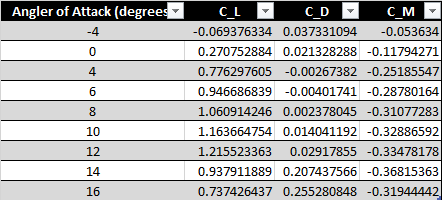
\includegraphics[width=10 cm]{CLCDCM.png}
        \centering
        \caption{Values for \(C_L\), \(C_D\), and \(C_M\)}
    \end{figure}

\newpage
\subsection{\(C_P\) Data}
    \begin{figure}[h]
        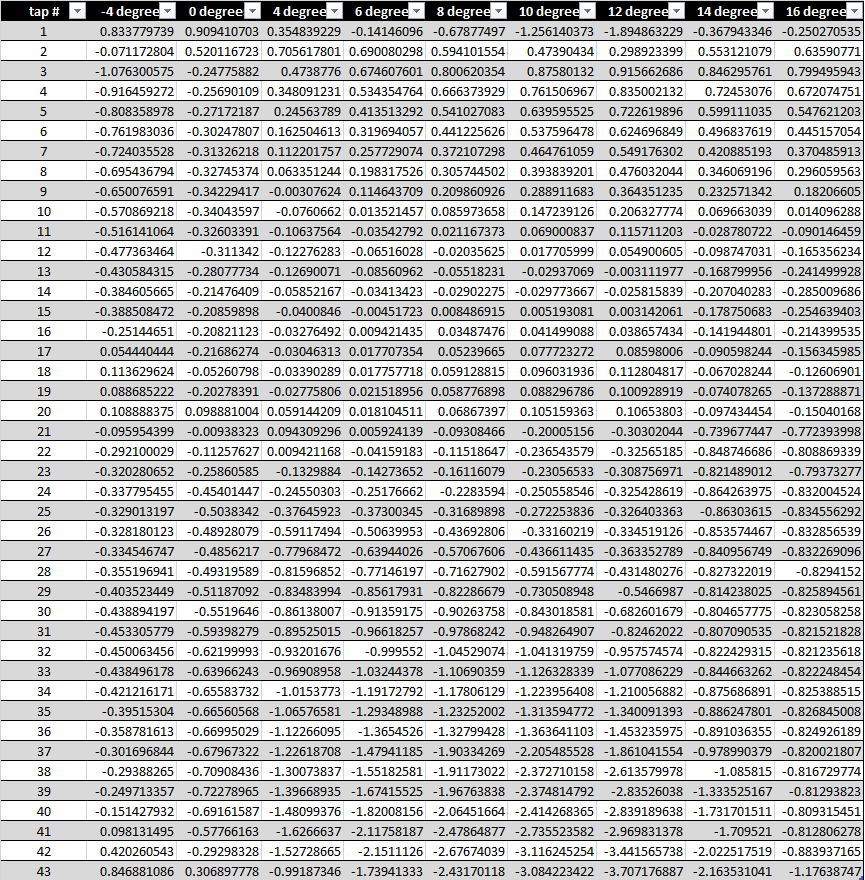
\includegraphics[width=16.2 cm]{cp.png}
        \centering
        \caption{\(C_P\) Data}
    \end{figure}
\newpage

\subsection{Estimated Location of Stagnation Point}
    \begin{figure}[h]
        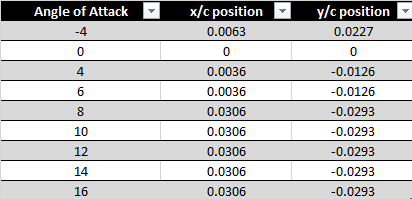
\includegraphics[width=10 cm]{pos.png}
        \centering
        \caption{Estimated Location of Stagnation Point}
    \end{figure}
\newpage

\subsection{Location of Pressure Taps on GA(W)-1 airfoil}
    \begin{figure}[h]
        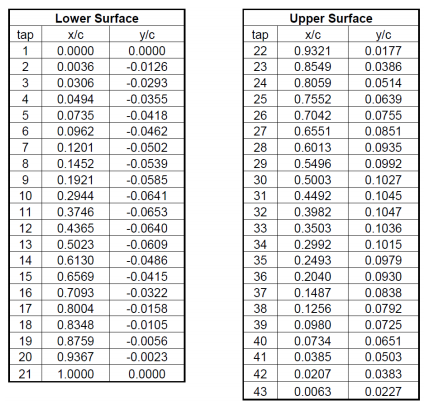
\includegraphics[width=10 cm]{location.PNG}
        \centering
        \caption{Location of Pressure Taps on GA(W)-1 airfoil}
    \end{figure}
\newpage


\section{Appendix of Matlab Code}
\subsection{Code for Plots and Data Manipulation}
\begin{lstlisting}
%344 Lab 4
clear, clc
%Create an array with all the averages
avg = zeros(9,45);
cphold = zeros(1,24);
% -4 degree
f5 = csvread('344Lab5Data\-4.csv');
i = 1; p = 1;
while (i < 44)
    avg(1,p) = mean(f5(:,i));
    i = i+1;
    p = p+1;
end
avg(1,44) = mean(f5(:,44));
avg(1,45) = mean(f5(:,45));

% 0 degree
f5 = csvread('344Lab5Data\0.csv');
i = 1; p = 1;
while (i < 44)
    avg(2,p) = mean(f5(:,i));
    i = i+1;
    p = p+1;
end
avg(2,44) = mean(f5(:,44));
avg(2,45) = mean(f5(:,45));

% 4 degree
f5 = csvread('344Lab5Data\4.csv');
i = 1; p = 1;
while (i < 44)
    avg(3,p) = mean(f5(:,i));
    i = i+1;
    p = p+1;
end
avg(3,44) = mean(f5(:,44));
avg(3,45) = mean(f5(:,45));

% 6 degree
f5 = csvread('344Lab5Data\6.csv');
i = 1; p = 1;
while (i < 44)
    avg(4,p) = mean(f5(:,i));
    i = i+1;
    p = p+1;
end
avg(4,44) = mean(f5(:,44));
avg(4,45) = mean(f5(:,45));

% 8 degree
f5 = csvread('344Lab5Data\8.csv');
i = 1; p = 1;
while (i < 44)
    avg(5,p) = mean(f5(:,i));
    i = i+1;
    p = p+1;
end
avg(5,44) = mean(f5(:,44));
avg(5,45) = mean(f5(:,45));

% 10 degree
f5 = csvread('344Lab5Data\10.csv');
i = 1; p = 1;
while (i < 44)
    avg(6,p) = mean(f5(:,i));
    i = i+1;
    p = p+1;
end
avg(6,44) = mean(f5(:,44));
avg(6,45) = mean(f5(:,45));

% 12 degree
f5 = csvread('344Lab5Data\12.csv');
i = 1; p = 1;
while (i < 44)
    avg(7,p) = mean(f5(:,i));
    i = i+1;
    p = p+1;
end
avg(7,44) = mean(f5(:,44));
avg(7,45) = mean(f5(:,45));

% 14 degree
f5 = csvread('344Lab5Data\14.csv');
i = 1; p = 1;
while (i < 44)
    avg(8,p) = mean(f5(:,i));
    i = i+1;
    p = p+1;
end
avg(8,44) = mean(f5(:,44));
avg(8,45) = mean(f5(:,45));

% 16 degree
f5 = csvread('344Lab5Data\16.csv');
i = 1; p = 1;
while (i < 44)
    avg(9,p) = mean(f5(:,i));
    i = i+1;
    p = p+1;
end
avg(9,44) = mean(f5(:,44));
avg(9,45) = mean(f5(:,45));

%-------------------------------------------------------------------------%
%-------------------------------------------------------------------------%
%-------------------------------------------------------------------------%

x = [0 0.0036 0.0306 0.0494 0.0735 0.0962 0.1201 0.1452 0.1921 0.2944 0.3746 0.4365 0.5023 0.613 0.6569 0.7093 0.8004 0.8348 0.8759 0.9367 1 0.9321 0.8549 0.8059 0.7552 0.7042 0.6551 0.6013 0.5496 0.5003 0.4492 0.3982 0.3503 0.2992 0.2493 0.204 0.1487 0.1256 0.098 0.0734 0.0385 0.0207 0.0063 0 ];
y = [0 -0.0126 -0.0293 -0.0355 -0.0418 -0.0462 -0.0502 -0.0539 -0.0585 -0.0641 -0.0653 -0.064 -0.0609 -0.0486 -0.0415 -0.0322 -0.0158 -0.0105 -0.0056 -0.0023 0 0.0177 0.0386 0.0514 0.0639 0.0755 0.0851 0.0935 0.0992 0.1027 0.1045 0.1047 0.1036 0.1015 0.0979 0.093 0.0838 0.0792 0.0725 0.0651 0.0503 0.0383 0.0227 0];


%-4
cp1 = ((avg(1,1:43)-avg(1,44))./(1.1.*(avg(1,45)-avg(1,44))));
figure(1)
plot(x(1:21), cp1(1:21));
set(gca, 'Ydir', 'reverse')
hold on 

cphold(1:23) = cp1(21:43);
cphold(24) = cp1(1);
plot(x(21:44), cphold(1:24))

title("C_p vs x/c");
xlabel("x/c");
ylabel("C_p");
legend("Bottom Surface","Top Surface")
hold off

%0
cp2 = ((avg(2,1:43)-avg(2,44))./(1.1.*(avg(2,45)-avg(2,44))));
figure(2)

plot(x(1:21), cp2(1:21));
set(gca, 'Ydir', 'reverse')
hold on 
cphold(1:23) = cp2(21:43);
cphold(24) = cp2(1);
plot(x(21:44), cphold(1:24))
title("C_p vs x/c");
xlabel("x/c");
ylabel("C_p");
legend("Bottom Surface","Top Surface")
hold off

%4
cp3 = ((avg(3,1:43)-avg(3,44))./(1.1.*(avg(3,45)-avg(3,44))));
figure(3)

plot(x(1:21), cp3(1:21));
set(gca, 'Ydir', 'reverse')
hold on 
cphold(1:23) = cp3(21:43);
cphold(24) = cp3(1);
plot(x(21:44), cphold(1:24))
title("C_p vs x/c");
xlabel("x/c");
ylabel("C_p");
legend("Bottom Surface","Top Surface")
hold off

%6
cp4 = ((avg(4,1:43)-avg(4,44))./(1.1.*(avg(4,45)-avg(4,44))));
figure(4)

plot(x(1:21), cp4(1:21));
set(gca, 'Ydir', 'reverse')
hold on 
cphold(1:23) = cp4(21:43);
cphold(24) = cp4(1);
plot(x(21:44), cphold(1:24))
title("C_p vs x/c");
xlabel("x/c");
ylabel("C_p");
legend("Bottom Surface","Top Surface")
hold off

%8
cp5 = ((avg(5,1:43)-avg(5,44))./(1.1.*(avg(5,45)-avg(5,44))));
figure(5)

plot(x(1:21), cp5(1:21));
set(gca, 'Ydir', 'reverse')
hold on 
cphold(1:23) = cp5(21:43);
cphold(24) = cp5(1);
plot(x(21:44), cphold(1:24))
title("C_p vs x/c");
xlabel("x/c");
ylabel("C_p");
legend("Bottom Surface","Top Surface")
hold off

%10
cp6 = ((avg(6,1:43)-avg(6,44))./(1.1.*(avg(6,45)-avg(6,44))));
figure(6)

plot(x(1:21), cp6(1:21));
set(gca, 'Ydir', 'reverse')
hold on 
cphold(1:23) = cp6(21:43);
cphold(24) = cp6(1);
plot(x(21:44), cphold(1:24))
title("C_p vs x/c");
xlabel("x/c");
ylabel("C_p");
legend("Bottom Surface","Top Surface")
hold off

%12
cp7 = ((avg(7,1:43)-avg(7,44))./(1.1.*(avg(7,45)-avg(7,44))));
figure(7)

plot(x(1:21), cp7(1:21));
set(gca, 'Ydir', 'reverse')
hold on 
cphold(1:23) = cp7(21:43);
cphold(24) = cp7(1);
plot(x(21:44), cphold(1:24))
title("C_p vs x/c");
xlabel("x/c");
ylabel("C_p");
legend("Bottom Surface","Top Surface")
hold off

%14
cp8 = ((avg(8,1:43)-avg(8,44))./(1.1.*(avg(8,45)-avg(8,44))));
figure(8)

plot(x(1:21), cp8(1:21));
set(gca, 'Ydir', 'reverse')
hold on 
cphold(1:23) = cp8(21:43);
cphold(24) = cp8(1);
plot(x(21:44), cphold(1:24))
title("C_p vs x/c");
xlabel("x/c");
ylabel("C_p");
legend("Bottom Surface","Top Surface")
hold off

%16
cp9 = ((avg(9,1:43)-avg(9,44))./(1.1.*(avg(9,45)-avg(9,44))));
figure(9)

plot(x(1:21), cp9(1:21));
set(gca, 'Ydir', 'reverse')
hold on 
cphold(1:23) = cp9(21:43);
cphold(24) = cp9(1);
plot(x(21:44), cphold(1:24))
title("C_p vs x/c");
xlabel("x/c");
ylabel("C_p");
legend("Bottom Surface","Top Surface")
hold off


%-------------------------------------------------------------------------%
%-------------------------------------------------------------------------%
%-------------------------------------------------------------------------%
deltax = zeros(1,43);
deltay = zeros(1,43);
x2 = [0 0.0036 0.0306 0.0494 0.0735 0.0962 0.1201 0.1452 0.1921 0.2944 0.3746 0.4365 0.5023 0.613 0.6569 0.7093 0.8004 0.8348 0.8759 0.9367 1 0.9321 0.8549 0.8059 0.7552 0.7042 0.6551 0.6013 0.5496 0.5003 0.4492 0.3982 0.3503 0.2992 0.2493 0.204 0.1487 0.1256 0.098 0.0734 0.0385 0.0207 0.0063];
y2 = [0 -0.0126 -0.0293 -0.0355 -0.0418 -0.0462 -0.0502 -0.0539 -0.0585 -0.0641 -0.0653 -0.064 -0.0609 -0.0486 -0.0415 -0.0322 -0.0158 -0.0105 -0.0056 -0.0023 0 0.0177 0.0386 0.0514 0.0639 0.0755 0.0851 0.0935 0.0992 0.1027 0.1045 0.1047 0.1036 0.1015 0.0979 0.093 0.0838 0.0792 0.0725 0.0651 0.0503 0.0383 0.0227];
x3 = zeros(1,43);
y3 = zeros(1,43);
p1 = zeros(1,43);
p2 = zeros(1,43);
p3 = zeros(1,43);
p4 = zeros(1,43);
p5 = zeros(1,43);
p6 = zeros(1,43);
p7 = zeros(1,43);
p8 = zeros(1,43);
p9 = zeros(1,43);


i=1;
while(i<43)
    
    deltax(i) = x2(i+1)-x2(i);
    deltay(i) = y2(i+1)-y2(i);
    x3(i) = 0.5*(x(i)+x(i+1));
    y3(i) = 0.5*(y(i)+y(i+1));
    p1(i) = 0.5*(avg(1,i) + avg(1,i+1));
    p2(i) = 0.5*(avg(2,i) + avg(2,i+1));
    p3(i) = 0.5*(avg(3,i) + avg(3,i+1));
    p4(i) = 0.5*(avg(4,i) + avg(4,i+1));
    p5(i) = 0.5*(avg(5,i) + avg(5,i+1));
    p6(i) = 0.5*(avg(6,i) + avg(6,i+1));
    p7(i) = 0.5*(avg(7,i) + avg(7,i+1));
    p8(i) = 0.5*(avg(8,i) + avg(8,i+1));
    p9(i) = 0.5*(avg(9,i) + avg(9,i+1));
    i = i+1;
    
    
end

    deltax(43) = x2(1)-x2(43);
    deltay(43) = y2(1)-y2(43);
    x3(43) = 0.5*(x(43)+x(1));
    y3(43) = 0.5*(y(43)+y(1));
    p1(43) = 0.5*(avg(1,43) + avg(1,1));
    p2(43) = 0.5*(avg(2,43) + avg(2,1));
    p3(43) = 0.5*(avg(3,43) + avg(3,1));
    p4(43) = 0.5*(avg(4,43) + avg(4,1));
    p5(43) = 0.5*(avg(5,43) + avg(5,1));
    p6(43) = 0.5*(avg(6,43) + avg(6,1));
    p7(43) = 0.5*(avg(7,43) + avg(7,1));
    p8(43) = 0.5*(avg(8,43) + avg(8,1));
    p9(43) = 0.5*(avg(9,43) + avg(9,1));

    N1 = sum(p1.*deltax);
    N2 = sum(p2.*deltax);
    N3 = sum(p3.*deltax);
    N4 = sum(p4.*deltax);
    N5 = sum(p5.*deltax);
    N6 = sum(p6.*deltax);
    N7 = sum(p7.*deltax);
    N8 = sum(p8.*deltax);
    N9 = sum(p9.*deltax);
    N = [N1 N2 N3 N4 N5 N6 N7 N8 N9];
    
    A1 = -sum(p1.*deltay);
    A2 = -sum(p2.*deltay);
    A3 = -sum(p3.*deltay);
    A4 = -sum(p4.*deltay);
    A5 = -sum(p5.*deltay);
    A6 = -sum(p6.*deltay);
    A7 = -sum(p7.*deltay);
    A8 = -sum(p8.*deltay);
    A9 = -sum(p9.*deltay);
    A = [A1 A2 A3 A4 A5 A6 A7 A8 A9];

    M1 = -sum((p1.*deltax).*x3)-sum((p1.*deltay).*y3);
    M2 = -sum((p2.*deltax).*x3)-sum((p2.*deltay).*y3);
    M3 = -sum((p3.*deltax).*x3)-sum((p3.*deltay).*y3);
    M4 = -sum((p4.*deltax).*x3)-sum((p4.*deltay).*y3);
    M5 = -sum((p5.*deltax).*x3)-sum((p5.*deltay).*y3);
    M6 = -sum((p6.*deltax).*x3)-sum((p6.*deltay).*y3);
    M7 = -sum((p7.*deltax).*x3)-sum((p7.*deltay).*y3);
    M8 = -sum((p8.*deltax).*x3)-sum((p8.*deltay).*y3);
    M9 = -sum((p9.*deltax).*x3)-sum((p9.*deltay).*y3);
    M = [M1 M2 M3 M4 M5 M6 M7 M8 M9];
    
    alpha = [-4 0 4 6 8 10 12 14 16];
    
    L = N.*cosd(alpha) - A.*sind(alpha);
    D = N.*sind(alpha) + A.*cosd(alpha);
    
    CL = L;
    CD = D;
    CM = M;
    i=1;
    while(i<10)
    CL(i)=(CL(i))./(1.1.*(avg(i,45)-avg(i,44)));
    CD(i)=(CD(i))./(1.1.*(avg(i,45)-avg(i,44)));
    CM(i)=(CM(i))./(1.1.*(avg(i,45)-avg(i,44)));
    i= i+1;
    end
    z2 = linspace(-4,16,40);
    %Lift
    figure(10)
    p1 = polyfit(alpha,CL,5);
    
    hold on
    plot(alpha, CL,"o")
    plot(z2, polyval(p1,z2))
    title("Lift Coefficent vs Angle of Attack");
    xlabel("Angle of Attack (\alpha in degrees)");
    ylabel("Lift Coefficent (C_L)");
    legend("Raw data","Best Fit")
    hold off

    %Drag
    figure(11)
    p2 = polyfit(alpha,CD,4); 
    hold on
    plot(alpha, CD,"o")
    plot(z2, polyval(p2,z2))
    title("Drag Coefficet vs Angle of Attack");
    xlabel("Angle of Attack (\alpha in degrees)");
    ylabel("Drag Coefficent (C_D)");  
    legend("Raw data","Best Fit")
    hold off
    
    %Moment
    figure(12)
    p3 = polyfit(alpha,CM,6); 
    hold on
    plot(alpha, CM,"o")
    plot(z2, polyval(p3,z2))
    title("Moment Coefficent vs Angle of Attack");
    xlabel("Angle of Attack (\alpha in degrees)");
    ylabel("Moment Coefficent");
    legend("Raw data","Best Fit")
    hold off




\end{lstlisting}



\end{document}
